\chapter{Meet The Most Interesting Man On The Planet}

These notes follow the School of Hard Knocks interview with Abdullah ``AK'' Kudrath, curated by LazyingArt LLC. The opening image is wealth: a Rolls-Royce, a Lamborghini Urus, a Ferrari 458, a Lamborghini Diablo. But the interview quickly asks a better question than ``who owns the car?'' It asks how a working emergency-room doctor turns direct labor into institutions, operating procedures, risk-bearing businesses, and a philosophy of money that still leaves health and character at the center.

\section{The Wealth Hook And The Actual Problem}

The lecture opens with a deliberately visible sign of success. The host asks whether the Rolls-Royce belongs to AK, then moves through the cars and into the claim that AK has built multiple eight-figure businesses while still saving lives on a weekly basis. That visual wealth is not the proof of the chapter. It is the hook that gets us to the real problem: how does one person move from doing valuable work directly to building systems that continue beyond the person?

The first useful quantities are modest orientation marks:
\begin{equation}
N_{\mathrm{companies}} > 7,
\end{equation}
where \(N_{\mathrm{companies}}\) is the number of companies attributed to AK in the host's introduction, and
\begin{equation}
T_{\mathrm{doctor}} \approx 7\text{--}8 \ \mathrm{years},
\end{equation}
the approximate length of AK's medical practice at the time of the interview. These are not valuation equations. They are coordinates: one coordinate says ``repeated company formation,'' and the other says ``continuing professional practice.''

AK's own inventory gives the first structural clue. He is formally trained as an emergency-room doctor and still works in emergency rooms. He began with emergency departments, built several of them, then created a physician group that hires doctors to work in outside hospitals. After that came other industries: a limo company, office space, real estate development, lake homes, a Botox and filler company, a lounge in Midtown, and smaller ventures.

We should read this list as a sequence, not merely as decoration. It starts close to medical competence, moves into the management of medical labor, and then steps outward into unrelated or semi-related commercial bets. The chapter is about the mechanism that makes that stepping-out possible.

\section{Health As The Limit On Wealth}

Before the interview turns to scaling, it asks what medicine has taught AK about people. His answer is the first correction to a money-only reading of the story. When health is on the line, people care about health.

The anecdote is concrete. AK says he has seen patients with millions of dollars, patients for whom money was arriving in large amounts, who nevertheless said that the money meant nothing because they wanted their body back. One patient with stomach cancer wished he could simply have his belly back.

This gives us a clean separation between anecdote, claim, and mechanism:
\begin{itemize}
\item Anecdote: a wealthy patient with stomach cancer would trade the money for health.
\item Claim: when health is threatened, health dominates money.
\item Mechanism: bodily crisis changes the priority ordering.
\end{itemize}

A compact way to record the priority reversal is
\begin{equation}
\mathrm{Priority}(\mathrm{health}\mid \mathrm{health\ crisis})
>
\mathrm{Priority}(\mathrm{money}\mid \mathrm{health\ crisis}).
\end{equation}
This is not a law of economics, and it should not be treated as one. It is a transcript-backed rule of judgment. The interview begins with cars, but its first serious lesson is that wealth has to be pursued inside a larger constraint: health, family, and the fact that the body can suddenly make every other ambition secondary.

\section{From One Doctor To Durable Institutions}

The turning point comes from AK's medical trip in East Africa. He went with a small church group to see people in villages, and he remembers the situation as one doctor with one medical bag. He says the work was meaningful for the people they saw. The number he gives is substantial:
\begin{equation}
P_{\mathrm{East\ Africa}} \approx 250 \ \mathrm{patients/day}.
\end{equation}
But the same number also reveals the ceiling. Even at roughly two hundred fifty patients a day, one doctor is still one person. There is a limit to what direct service can touch.

\subsection{Question \& Answer}

\paragraph{Question.}
Why was being one doctor with a medical bag not enough?

\paragraph{Answer.}
Because direct service can be meaningful without being structurally sufficient. AK's phrase is that he could barely scratch the surface of any real problem. The conclusion he draws is not that medicine is unimportant. It is that institutions and operations can outlast the individual worker:
\begin{equation}
\mathrm{Durability}(\mathrm{institution})
>
\mathrm{Durability}(\mathrm{individual\ labor}).
\end{equation}

This is the first true scaling idea in the lecture. We begin with a person doing necessary work. Then we ask what remains when that person is absent, tired, sick, or gone. AK's answer is not charisma. It is the building of facilities, systems, and organizations that can keep acting after one person's shift is over.

\section{The Operating System Of Scale}

The host then makes the pivot explicit: AK has brought up scaling, and scaling is where many entrepreneurs struggle. The question is how to take a business from six figures to seven figures. AK answers with a capacity argument.

If the owner does everything personally, the business is bounded by the owner's available hours. Let \(H_{\mathrm{owner}}\) denote the owner's usable work capacity and \(C_{\mathrm{owner}}\) the capacity of a business still dependent on that owner's direct task execution. Then the first approximation is
\begin{equation}
C_{\mathrm{owner}} \leq H_{\mathrm{owner}}.
\end{equation}
That inequality is the practical obstacle. A business cannot scale indefinitely if every crucial task must pass through one human schedule.

AK's clothing-store example makes the point. A friend has a successful store and is there all the time. But how can he open more locations if no one else can work the store? And how can anyone else work the store if the owner does not know how to select people or train people?

The mechanism is therefore not merely ``hire someone.'' It is a sequence:
\begin{enumerate}
\item identify repeatable work;
\item write the work down as standard operating procedures;
\item select people capable of doing parts of the work;
\item train those people;
\item supervise the managers and the organization;
\item provide the information, tools, benefits, and inspiration that keep the system alive.
\end{enumerate}

A cautious capacity shorthand is
\begin{equation}
C_{\mathrm{scaled}}
\sim
C_{\mathrm{owner}}
+
\sum_{i=1}^{n} C_{\mathrm{operator},i},
\end{equation}
where \(C_{\mathrm{operator},i}\) is the reliable capacity of the \(i\)-th trained operator. The symbol \(\sim\) matters. This is not a financial formula from the interview. It is a note-writing reconstruction of AK's mechanism: capacity increases when trained people can carry repeatable work under procedures and supervision.

\begin{figure}
\centering
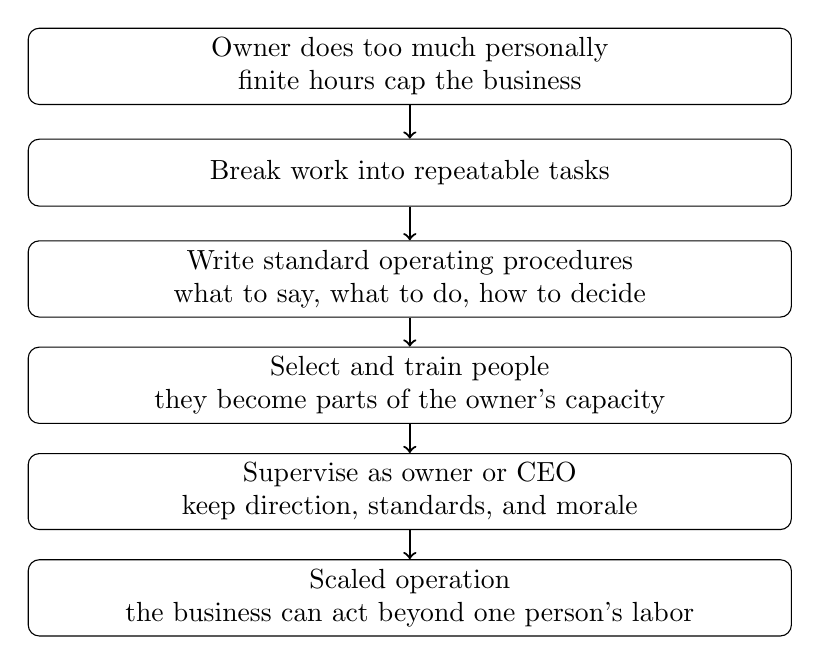
\begin{tikzpicture}[
box/.style={draw, rounded corners, align=center, text width=0.78\linewidth, minimum height=0.85cm},
arrow/.style={->, thick}
]
\node[box] (limit) at (0,0) {Owner does too much personally\\finite hours cap the business};
\node[box] (tasks) at (0,-1.35) {Break work into repeatable tasks};
\node[box] (sop) at (0,-2.70) {Write standard operating procedures\\what to say, what to do, how to decide};
\node[box] (people) at (0,-4.05) {Select and train people\\they become parts of the owner's capacity};
\node[box] (supervise) at (0,-5.40) {Supervise as owner or CEO\\keep direction, standards, and morale};
\node[box] (scale) at (0,-6.75) {Scaled operation\\the business can act beyond one person's labor};
\draw[arrow] (limit) -- (tasks);
\draw[arrow] (tasks) -- (sop);
\draw[arrow] (sop) -- (people);
\draw[arrow] (people) -- (supervise);
\draw[arrow] (supervise) -- (scale);
\end{tikzpicture}
\caption{Transcript-grounded reconstruction of AK's scaling mechanism: finite owner time must be converted into repeatable procedures, trained people, and continuing leadership.}
\end{figure}

\subsection{Question \& Answer}

\paragraph{Question.}
Is a standard operating procedure enough to scale?

\paragraph{Answer.}
No. AK names SOPs as a requirement, but he immediately adds the limitation. No one will run the company exactly the way the founder runs it. Even with the same procedures, leadership changes can damage a company. The owner or CEO still has to supervise direction, inspire managers, and make sure people have the right information and tools.

Thus the practical mechanism is better written as
\begin{equation}
\mathrm{Scale}
=
f(\mathrm{SOPs},\mathrm{selection},\mathrm{training},\mathrm{supervision}).
\end{equation}
The warning is that leaving out the final terms changes the result. Procedures without leadership are brittle. Leadership without procedures is trapped inside one person.

\section{Risk, The First Business, And The First Million}

The interview then turns from operating systems to motivation. AK's father told him, when he was entering medical school, that if he did it only for himself, then falling down might become comfortable. But if he carried the flag of family, community, country, or world, then falling down would not be the end. He would look up, see what he was carrying, and get back up.

That advice becomes the motivational side of risk. When asked about the most money he made in a single year, AK resists precision. He says there are good years and bad years, that people may hear ``a couple million'' and misunderstand, and that taxes and reinvestment matter. The safe transcript-backed notation is
\begin{equation}
I_{\mathrm{best\ year}} \approx \hbox{``a couple million''},
\end{equation}
with the immediate qualification
\begin{equation}
\mathrm{Spendable\ income} \neq \mathrm{gross\ income}.
\end{equation}
Taxes and reinvestment reduce what can be treated as available personal spending. This is why the money answer should not become a headline detached from the operating context.

When asked for the best financial decision he ever made, AK answers: the first one, the first business. He invokes the saying that the first million is the hardest, because once one has money, one has comfort and can start investing in other projects. But the transcript does not turn this into romance about risk. It gives a discipline.

\subsection{A Worked Risk Rule}

Let \(K\) be capital available for a first serious business move. Let \(L\) be the possible loss, \(B\) the backup plan, and \(R\) the reinvestment needed for growth. AK's rule is not ``maximize the bet.'' It is closer to a survival-constrained update:
\begin{align}
K &\longrightarrow \hbox{capital saved for the first move},\\
L &\longrightarrow \hbox{downside estimated in advance},\\
B &\longrightarrow \hbox{backup plan kept alive},\\
R &\longrightarrow \hbox{cash reserved or returned to growth}.
\end{align}
The decision rule is:
\begin{equation}
\hbox{Take the risk only if } L \hbox{ is survivable and } B \hbox{ is real.}
\end{equation}
Then the work begins. AK's language is that one has to lose the ego and do whatever it takes to make sure the ship does not sink.

The learning update after a difficult attempt is:
\begin{equation}
\mathrm{Skill}_{t+1}
=
\mathrm{Skill}_{t}
+
\Delta(\mathrm{attempt},\mathrm{loss},\mathrm{correction}).
\end{equation}
This is a standard reconstruction of his spoken claim: sometimes one loses, sometimes one wins, but without trying one never learns the skill set needed to keep growing.

\section{Accountability And The Stages Of The Entrepreneurial Problem}

The next question asks for the secret to self-improvement. AK again returns to his father. The rule is: never point fingers. There is always blame to go around, but the useful question is what one could have done differently.

This is a learning algorithm. If a project fails and the only output is blame, the operator does not improve. If the same failure is converted into a better selection rule, a better training rule, more background work, or harder execution, then failure has become information.

A compact way to write the rule is
\begin{equation}
\mathrm{Growth}
\propto
\mathrm{Accountability}
\times
\mathrm{Correction}.
\end{equation}
If accountability is zero, correction rarely begins. This is why AK says that if one always thinks everybody else did everything wrong, one never gets better.

AK's answer about entrepreneurial challenge then widens the same logic into stages. The early challenge is getting started: knowledge, money, and the character not to squander what is handed over. He gives a hypothetical example:
\begin{equation}
C_{\mathrm{starter}}=\$1{,}000{,}000.
\end{equation}
Even if someone receives a million dollars and the books or teaching needed to begin, AK says many will still fail because they become greedy, emotional, unreliable, idle, or unable to meet deadlines.

The next challenge is diversification. The stakes grow. A first move may require tens or hundreds of thousands. Later, one may be betting around a million dollars and risking what earlier work created. Then the challenge becomes risk calculation.

The final challenge is balance after success. AK states the thought experiment:
\begin{equation}
W_{\mathrm{retirement}}=\$10{,}000{,}000.
\end{equation}
At that point a person might be able to retire, but may not be built to stop. The real question becomes how to put life together: relationships, children, parents, and time.

\begin{table}
\centering
\begin{tabular}{|p{0.24\linewidth}|p{0.31\linewidth}|p{0.31\linewidth}|}
\hline
Stage & Main Question & Common Failure Mode \\
\hline
Starting & How do I get knowledge and money? & Never beginning, or beginning without a plan \\
\hline
Character & Can I be trusted with opportunity? & Greed, emotion, missed deadlines, idleness \\
\hline
Diversifying & Should I bet bigger now or later? & Mispriced risk and financial ruin \\
\hline
Post-success & What is life for after enough money? & Losing family, health, or balance \\
\hline
\end{tabular}
\caption{AK's staged account of entrepreneurial difficulty. The problem changes as capital, competence, and optionality increase.}
\end{table}

\section{Reputation, History, And What Money Is For}

The last part of the interview broadens the lens. Asked whom he would spend a day with, AK names Benjamin Franklin. The point of the answer is reputation and diplomacy. AK admires Franklin as an inventor, statesman, and diplomat, and he frames him as someone respected enough that different powers would come back to the table when he spoke. We should preserve this as AK's admiration and claim, not expand it into independent historical proof.

The mechanism AK extracts is simple: make something of yourself, be honest, treat people fairly, and become the kind of person whose words are worth hearing. In the language of these notes:
\begin{equation}
\mathrm{Influence}
\approx
g(\mathrm{competence},\mathrm{honesty},\mathrm{fairness},\mathrm{trust}).
\end{equation}
This is the same structure as the business lesson, but applied to public life. Capacity is not only labor capacity. There is also trust capacity: the ability to convene, persuade, and calm conflict because people believe one is not merely extracting from them.

The world-history answer continues the theme. AK says humans keep being fooled by the same tricks: people seeking power divide others, sell narratives, provoke emotional decisions, and make people fight over hard ideological lines. The practical lesson is not cynicism. It is constructive judgment: understand why the other side sees what it sees, then ask what can be done to make things better.

The final question returns to his father. The greatest lesson is not to get caught up with the money. AK offers a final identity experiment:
\begin{equation}
W_{\mathrm{identity}}=\$100{,}000{,}000.
\end{equation}
Suppose that money is taken away. What remains? The answer he wants to preserve is not the account balance, but the person: whether others still say that he helped, looked out for people, was a good friend, and was a good family member.

This is the closing invariant of the interview. Money can vary. Businesses can vary. The protected quantity is the person who remains after acquisition, success, and influence.

\section{Summary}

The interview begins with cars, but it does not end there. Its real arc is a theory of conversion: direct professional labor becomes durable institutions through operations; owner capacity becomes organizational capacity through SOPs, selection, training, and supervision; risk becomes skill when it is calculated and survived; failure becomes growth when it is met with accountability; and money becomes dangerous if it replaces health, family, reputation, and character.

For the larger book, AK's contribution is strongest on five durable questions: what a person actually controls, how scale is built, how risk is financed and survived, which operating discipline compounds fastest, and what wealth is for after the number is reached. His answer is that money should remain a byproduct of useful work and personal growth. The protected asset is the person who remains after the money arrives.